\chapter{A Guideline for Developers}
\lipsum[1-1]


\section{Use \forkOn for embarrassingly parallel problems}
\sstate{Description:} Both the performance and energy consumption of a program can be improved by using \forkOn to create new threads of execution when there is little or no dependency among these threads and they perform almost the same amount of work.
\newline

\sstate{Rationale:} A problem that can be decomposed into parallel tasks that do not need to communicate with each other to make progress is called \emph{embarrassingly parallel}~\cite{herlihy:2012}. Three of the benchmarks from \chapref{chp:study} fits this description: \mandelbrot, \regex and \spectral. The results from our study has shown that, for these benchamrks, the variants using \forkOn superseded the others in both performance and energy consumption. This result shows that manually distributing the workload in an even manner among the capabilities instead of handing this job to the runtime system scheduler improves performance. It makes sense because we know before hand that each worker thread is doing exactly the same amount of work. In such scenarios, there is no need for migrating a thread from one capability to another since an even distribution is the one which contributes the most for the program's progress. It makes sure that each capability will have the same workload. So using \forkOn in these cases reduces the overhead incurred by the Haskell runtime system.

\begin{figure*}[tp]
\caption{Performence of \mandelbrot and \spectral with different number of workers}
\centering
$
\begin{array}{ccc}
 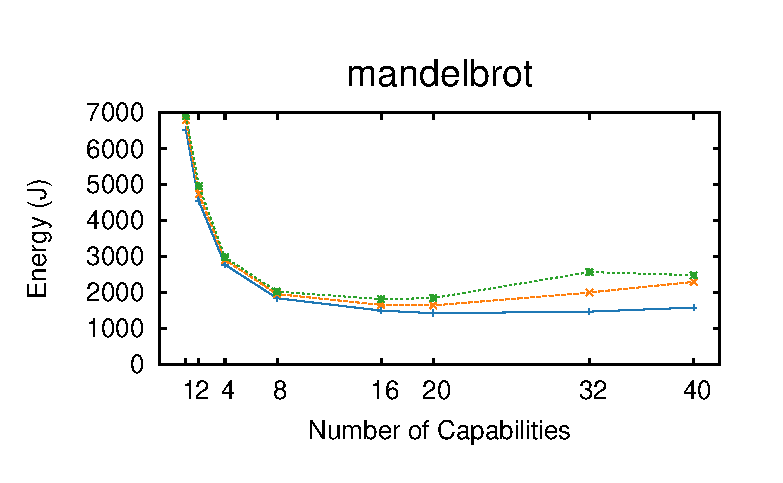
\includegraphics[width=.48\textwidth]{images/conc_bench/mandelbrot-Xt-energy} &
 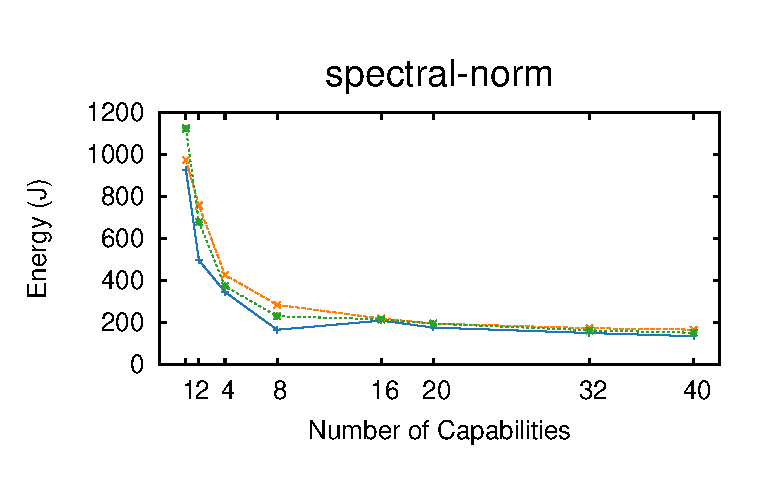
\includegraphics[width=.48\textwidth]{images/conc_bench/spectral-norm-Xt-energy} \\

 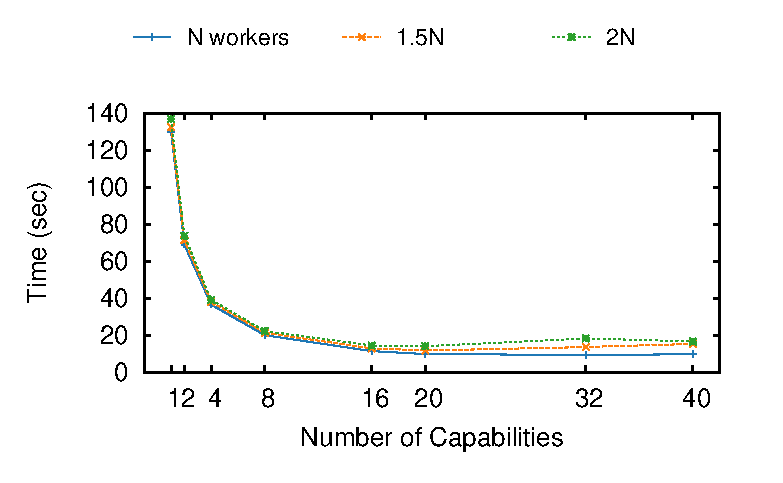
\includegraphics[width=.48\textwidth]{images/conc_bench/mandelbrot-Xt-time} &
 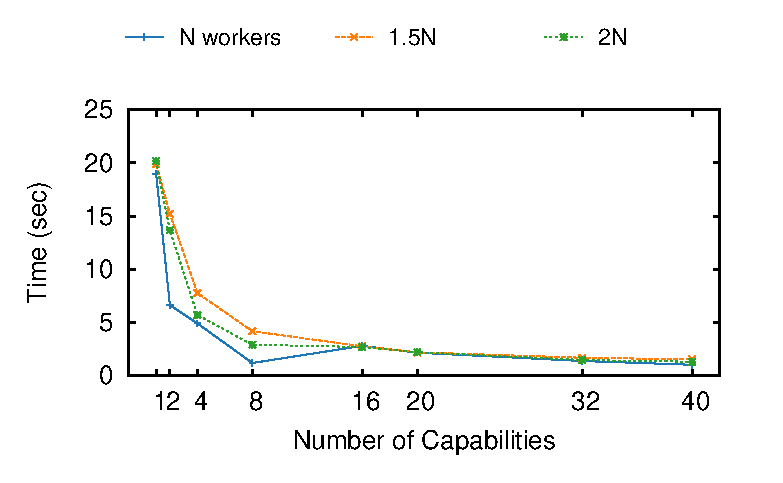
\includegraphics[width=.48\textwidth]{images/conc_bench/spectral-norm-Xt-time} \\
\end{array}
$
\footnotesize{Source: Made by the author}
\label{fig:more-threads}
\end{figure*}

However, \regex is implemented diffenrently from \mandelbrot and \spectral. The first one uses a fixed number of worker threads (350) while the others the number of threads can be set by the developer. For the experiments of \chapref{chp:study}, we set these benchmarks to spawn as many threads as the number of capabilities. We decided to run another experiment with \mandelbrot and \spectral to check how they behave if we overpopulate the capabilities' work queue. In \figref{fig:more-threads}, we can see the results for the \forkOn-\MVar variant of both benchmarks with $N$, $1.5N$ and $2N$ worker threads, where $N$ is the number of capabilities. As we can see, although the performance is similar, one thread per capability is the configuration with the best performance. This result makes sense because it reduces the costs of context-switching between threads of the capabilities' work queue. Thus, creating one worker thread per capability benefits both performance and energy consumption.

\begin{figure*}[tp]
\caption{Performence of \regex and \spectral using \texttt{-qa} and \texttt{-qm}}
\centering
$
\begin{array}{ccc}
 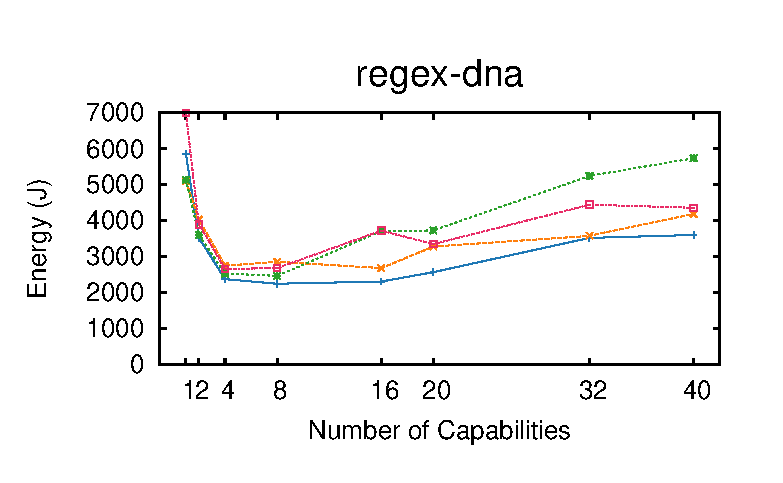
\includegraphics[width=.48\textwidth]{images/conc_bench/regex-dna-qX-energy} &
 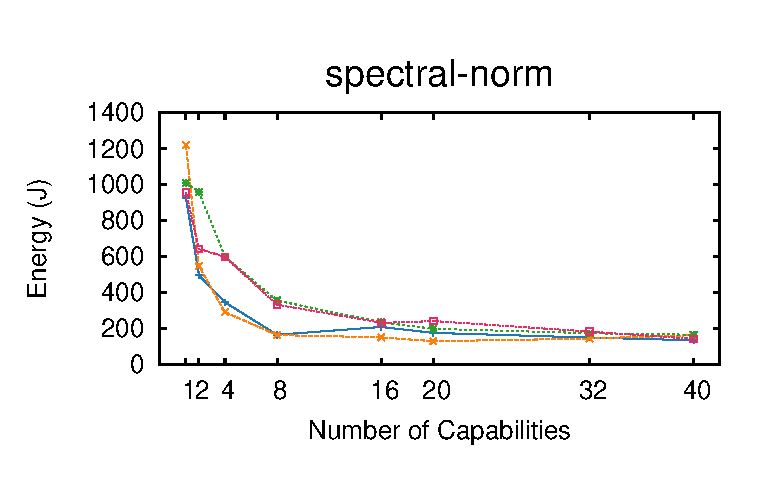
\includegraphics[width=.48\textwidth]{images/conc_bench/spectral-norm-qX-energy} \\

 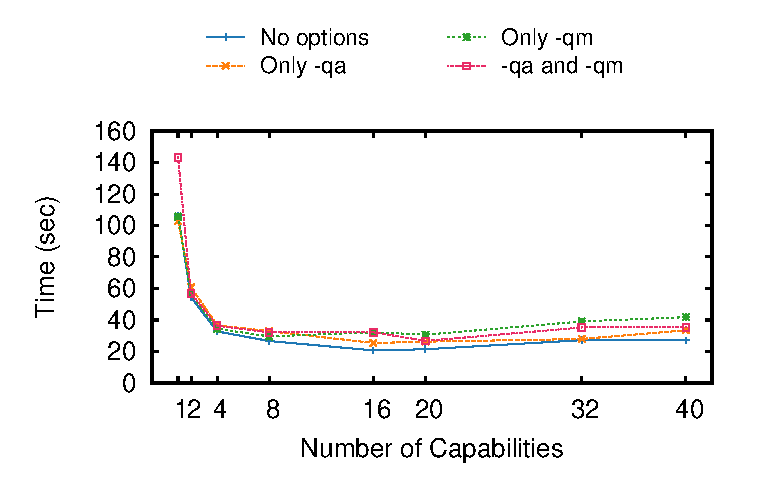
\includegraphics[width=.48\textwidth]{images/conc_bench/regex-dna-qX-time} &
 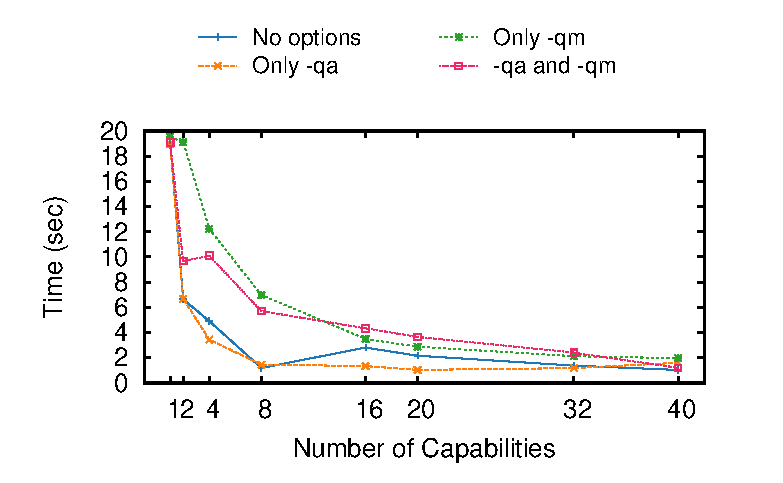
\includegraphics[width=.48\textwidth]{images/conc_bench/spectral-norm-qX-time} \\
\end{array}
$
\footnotesize{Source: Made by the author}
\label{fig:rts-flags}
\end{figure*}

Additionally, there are two \ac{rts} options that, in conjunction with \forkOn, can affect the performance of some embarrassingly parallel algorithms. The first one is the \texttt{-qa} option. It tries to pin OS threads to CPU cores using native OS facilities\footnote{In Linux, GHC uses the \texttt{sched\_setaffinity()} syscall}. Using this option, the OS threads associated with a capability \emph{i} are bound the CPU core \emph{i}. The other one is the \texttt{-qm} option. It disables automatic migration of threads between CPUs. The former seems to fit perfectly in this context since it increases the probability of a Haskell thread being kept running on the same CPU core during the execution of the program. However, it is not clear how different the latter is from simply creating all threads with \forkOn as we are proposing here. To get a picture of their influence, we executed our embarrassingly parallel benchmarks with these options. In \figref{fig:rts-flags} we show results for the \forkOn-\MVar variant of both \regex and \spectral. Here, we executed the benchmarks without either of the options, only with \texttt{-qa}, only with \texttt{-qm}, and with both options. As we can see, the \ac{rts} options affect the performance of both benchmarks. However, the behavior is not predictable. In \spectral, using only \texttt{-qa} improves both performance and energy consumption regardless of the number of capabilities. In \regex, however, using any combination of the \ac{rts} options has a negative impact on performance. It also increases considerably the energy consumption for more than eight capabilities. We recommend developers to experiment with these options to assess how they affect the performance of a given program.

\section{Avoid setting more capabilities than available CPUs}
\sstate{Description:} Using more capabilities than the number of available virtual CPU cores can seriously degrade both performance and energy consumption of a concurrent Haskell program.
\newline

\sstate{Rationale:} A capability is thought to act as an abstraction of a CPU for the Haskell runtime system. It is the entity that can execute Haskell code. This definition implies that we can achieve maximum parallelization by creating as many capabilities as the number of CPUs. In fact, this is precisely what the official \ac{ghc} documentation recommends for developers: to set \texttt{N} to be the same as the number of the processor's CPU cores. In our experiments from \chapref{chp:study}, we analyzed how each benchmark behaved for different capabilities settings. The results have shown that, for most benchmarks, the performance improved as we added more capabilities. It also confirmed the intuition that it does not make sense to outnumber the CPU cores. For eight of our benchmarks, both the performance and energy consumption were severely impaired by going from \texttt{N=40} to \texttt{N=64}.

However, modern Intel processors are equipped with a feature called \emph{hyperthreading}. This technology increases the number of independent instructions in the processor's pipeline. For each processor core that is physically present, the operating system addresses two separate virtual cores. So from the developer's point of view, there is twice the number of CPU cores available. In this context, the \ac{ghc} documentation leaves as an open question if virtual cores should be accounted: \emph{"Whether hyperthreading cores should be counted or not is an open question; please feel free to experiment and let us know what results you find."}\footnote{\url{http://downloads.haskell.org/~ghc/7.10.2/docs/html/users\_guide/using-smp.html\#ftn.idp12916656}}. In our experiments, only one benchmark presented a significant improvement in both performance and energy consumption when going from \texttt{N=20} to \texttt{N=40}. All the others were negatively impacted by this change, which suggests that, in general, virtual cores should not be accounted for setting the number of capabilities.


\section{Avoid using \forkOS to spawn new threads}
\sstate{Description:} Using \forkOS undeliberately to spawn new threads of execution can degrade both performance and energy consumption of a concurrent Haskell program.
\newline

\sstate{Rationale:} A call to \forkOS creates a bound thread. From a high-level perspective, it works the same way as an unbound thread created via \forkIO or \forkOn. They are treated as regular Haskell threads by the runtime system scheduler. However, bound threads are executed differently from the unbound ones. Each bound thread is associated with its own OS thread. So the capability has to switch OS threads when it is time to execute a bound thread. The motivation for having this kind of thread is to support interoperability with native libraries that use thread-local state. This is the scenario where the Haskell documentation recommends the use of \forkOS. In our experiments from \chapref{chp:study}, we analyzed how each benchmark behaved if the worker threads were bound threads. The results show that none of the benchmarks benefited from using \forkOS instead of \forkIO or \forkOn. Both performance and energy consumption degrades considerably when we use bound threads. Probably, this degradation is associated with the overhead of switching OS threads. In our benchmarks, as all threads were created using the same primitive, there is a lot of bound threads and each capability has to frequently switch OS threads in order to execute the scheduled action. So based on these results, we recommend developers to avoid using \forkOS unless it is strictly required like for calling foreign functions.
